\documentclass[10pt]{article}
\usepackage{titlesec}
\usepackage{geometry}
\geometry{verbose,tmargin=.9in,bmargin=.9in,lmargin=1.0in,rmargin=1.0in}
\usepackage{amsmath,amsfonts,amsthm,amssymb}
\usepackage{url}
\usepackage{color}
\usepackage[usenames,dvipsnames,svgnames,table]{xcolor}
\usepackage[colorlinks=true, linkcolor=red, urlcolor=blue, citecolor=gray]{hyperref}
\usepackage{float}
\usepackage{caption}
\usepackage{subcaption}
\usepackage{graphicx}
\usepackage{wrapfig}
\usepackage{booktabs}
\usepackage{longtable}
\usepackage{enumerate}
\usepackage{multicol}
\usepackage{etoolbox}
\newcommand{\bs}[1]{\boldsymbol{#1}}
\newcommand{\bv}[1]{\mathbf{#1}}
\usepackage{listings}
\usepackage{bbm}

\definecolor{nyuDarkPurple}{HTML}{330662}
\definecolor{nyuOfficialPurple}{HTML}{57068c}

\newcommand{\spara}[1]{\vspace{.5em}\noindent {\large\sffamily\textcolor{nyuOfficialPurple}{#1}}}
\titleformat{\section}[hang]{\Large\sffamily\color{nyuDarkPurple}}{\thesection}{1em}{}
\titleformat{\subsection}[hang]{\large\sffamily\color{nyuDarkPurple}}{\thesection}{1em}{}
\titleformat{\subsubsection}[hang]{\normalsize\sffamily\color{gray}}{\thesection}{1em}{}

\usepackage{fancyhdr}
\pagestyle{fancy}
\lhead{
\includegraphics[width=4cm]{tandon_long_color.eps}}
\rhead{\thepage}
\pagenumbering{gobble}

\setcounter{secnumdepth}{0}

% math commands
\DeclareMathOperator{\R}{\mathbb{R}}
\newcommand{\E}{\mathbb{E}}

\begin{document}
	
\begin{center}
	\normalsize
	New York University Tandon School of Engineering
	
	Computer Science and Engineering
	\medskip
	
	\large
	CS-UY 4563: Written Homework 4. 
	
	Due Monday,  April 20th, 2020, 11:59pm.
	\medskip
	
	\normalsize 
	\noindent \emph{Collaboration is allowed on this problem set, but solutions must be written-up individually. Please list the names of any collaborators at the top of your solution set, or write ``No Collaborators" if you worked alone.}
	\medskip
\end{center} 

\subsection{Problem 1: Kernels for Shifted Images (20pts)}
In class we discussed why the Gaussian kernel is a better similarity metric for MNIST digits than the inner product. Here we consider an additional modification to the Gaussian kernel.

For illustration purposes we consider 5x5 black and white images: a pixel has value $1$ if it is white and value $0$ if it is black. For example, consider the following images of two 0s and two 1s:
\begin{align*}
I_1 &= \begin{bmatrix}
0 & 0 & 0 & 0 & 0 \\
0 & 1 & 1 & 1 & 0 \\
0 & 1 & 0 & 1 & 0 \\
0 & 1 & 1 & 1 & 0 \\
0 & 0 & 0 & 0 & 0 
\end{bmatrix} 
& I_2 &= \begin{bmatrix}
0 & 0 & 0 & 0 & 0 \\
0 & 0 & 1 & 0 & 0 \\
0 & 0 & 1 & 0 & 0 \\
0 & 0 & 1 & 0 & 0 \\
0 & 0 & 0 & 0 & 0 
\end{bmatrix} 
& I_3 &= \begin{bmatrix}
0 & 0 & 0 & 0 & 0 \\
1 & 1 & 1 & 0 & 0 \\
1 & 0 & 1 & 0 & 0 \\
1 & 1 & 1 & 0 & 0 \\
0 & 0 & 0 & 0 & 0 
\end{bmatrix} 
& I_4 &= \begin{bmatrix}
0 & 0 & 0 & 0 & 0 \\
0 & 0 & 0 & 1 & 0 \\
0 & 0 & 0 & 1 & 0 \\
0 & 0 & 0 & 1 & 0 \\
0 & 0 & 0 & 0 & 0 
\end{bmatrix}
\end{align*}

\begin{enumerate}[(a)]
	\item Let $\vec{x}_i \in \{0,1\}^{25}$ denote the vectorized version of image $I_i$, obtained by concatenating the rows of the matrix representation of the image into a vector. Compute a $4\times 4$ kernel matrix $\bv{K}$ for images $I_1, \ldots, I_4$ using the standard Gaussian kernel $k_G(I_i, I_j) = e^{-\|\vec{x}_i - \vec{x}_j\|_2^2}$. 

	\item Suppose $I_1$ and $I_2$ are in our training data and $I_3$ and $I_4$ are in our test data. Which training image is most similar to each of our test images according to Gaussian kernel similarity? Do you expect a kernel classifier ($k$-NN, kernel logistic regression, etc.) to correctly or incorrectly classify $I_3$ and $I_4$?
	
	
	\item Consider a ``left-right shift'' kernel, which is a similarity measure defined as follows:
	
	For an image $I_i$, let $I_i^{\text{right}}$ be the image with its far right column removed and let $I_i^{\text{left}}$ be the image with its far left column removed. Intuitively, $I_i^{\text{right}}$ corresponds to the image shifted one pixel to the right and $I_i^{\text{left}}$ corresponds to the image shifted one pixel left. Define a new similarity metric $k_{\text{shift}}$ as follows: 
	\begin{align*}
	k_{\text{shift}}(I_i, I_j) = k_G(I_i^\text{right}, I_j^\text{right}) + k_G(I_i^\text{left}, I_j^\text{left}) + k_G(I_i^{\text{right}}, I_j^{\text{left}}) + k_G(I_i^{\text{left}}, I_j^{\text{right}}) 
	\end{align*}
	Intuitively this kernel captures similarity between images which are similar \emph{after a shift}, something the standard Gaussian kernel does not account for. 
	
	Recompute the a $4\times 4$ kernel matrix $\bv{K}$ for images $I_1, \ldots, I_4$ using $k_{\text{shift}}$. 
	
	\item Again $I_1$ and $I_2$ were in our training data and $I_3$ and $I_4$ were in our test data. Now which training image is most similar to each of our test images according to the ``left-right shift'' kernel? Do you expect a typically kernel classifier to correctly or incorrectly classify $I_3$ and $I_4$?
	
	\item Prove that $k_{\text{shift}}$ is a positive semi-definite kernel function. \textbf{Hint:} Use the fact that $k_G$ is positive semi-definite.
\end{enumerate}

\subsection{Problem 2: Thinking About Margin (10pts)}
Consider the data set of four examples $\vec{x}_1, \ldots \vec{x}_4$ with two features each: $\vec{x}_i = (\vec{x}_i[1], \vec{x}_i[2])$. Each data example has a binary class
label $y_i=\pm 1$.

\begin{center}
	\begin{tabular}{|c|c|c|c|c|c|} \hline
		$x_{i}[1]$ & 0 & 1 & 1 & 2 \\ \hline
		$x_{i}[2]$ & 0 & 0.3 & 0.7 & 1 \\ \hline
		$y_i$ & -1 & -1 & 1 & 1 \\ \hline
	\end{tabular}
\end{center}

\begin{enumerate}[(a)]
	\item Find a linear classifier that separates the two classes.
	Your classifier $f$ should be of the form:
	\begin{align*}
	f(\vec{x}) = \begin{cases}
	1 & \text{if } b + w_1 \vec{x}[1] + w_2 \vec{x}[2] > 0 \\
	-1 & \text{if } b + w_1 \vec{x}[1] + w_2 \vec{x}[2] \leq 0
	\end{cases}
	\end{align*}
	State the intercept $b$ and weights $w_1$ and $w_2$ for your classifier.
	Note there is no unique correct answer, as there are multiple linear classifiers
	that could separate the classes.
	
	\item For the classifier you found in part (a), what is the maximum $\gamma$ such that
	\begin{align*}
	y_i(b+w_1x_{i1} + w_{2}x_{i2}) \geq \gamma, \mbox{ for all } i?
	\end{align*}
	
	\item Compute the margin of your classifier from part (a). The margin $m$ is the minimum perpendicular distance from any point to the separating hyperplane defined by a linear classifier. Mathematically it can be computed as:
	\begin{align*}
	m = \frac{\gamma}{\|\vec{w}\|_2},
	\end{align*}
	where $\|w\|_2 = \sqrt{w_1^2 + w_2^2}$.
	
	\item Which data examples are on the margin for your classifier? I.e. for which $i$ does $\vec{x}_i$ lie exactly distant $m$ from your chosen separating hyperplane?	
	
	\item Is your classifier a maximum margin classifier, or does there exists a separating hyperplane with larger margin? Justify your answer briefly (in words or math). To answer this question, it might be helpful to plot the dataset and your classification rule. 
\end{enumerate}

\subsection{Problem 3: Neural Networks for Curve Fitting (15pts)}
Consider the following 2-layer, feed forward neural network for single variate regression:
\begin{center}
	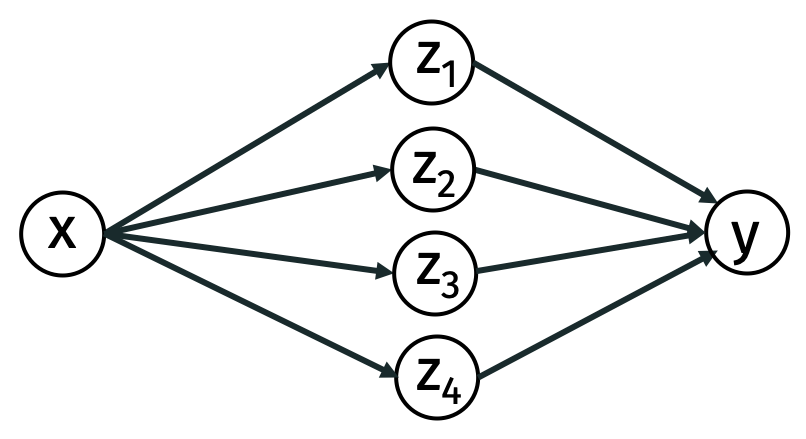
\includegraphics[width=.3\textwidth]{simple_net.png}
\end{center}
Let $W_{H,1}, W_{H,2}, W_{H,3}, W_{H,4}$ and $b_{H,1}, b_{H,2},b_{H,3},b_{H,4}$ be weights and biases for the hidden layer. Let $W_{O,1}, W_{O,2}$, $W_{O,3}, W_{O,4}$ and $b_{O}$ be weights and bias for the output layer. The hidden layer uses rectified linear unit (ReLU) non-linearities and the output layer uses no non-linearity.

Specifically, for $i = 1,\ldots, 4$, $z_i = \max(0,\bar{z}_i)$ where $\bar{z}_i = W_{H,i}x + b_{H,i}$. And
\begin{align*}
{y} = b_{O} + \sum_{i=1}^4 W_{O,i}z_i.
\end{align*}
\begin{enumerate}[(a)]
	\item For each of the two datasets below, determine values for weights and biases which would allow this network to perfectly fit the data.
	\captionsetup[subfigure]{labelformat=empty}
	\begin{figure}[h]
		\centering
		\begin{subfigure}{0.45\textwidth}
			\centering
			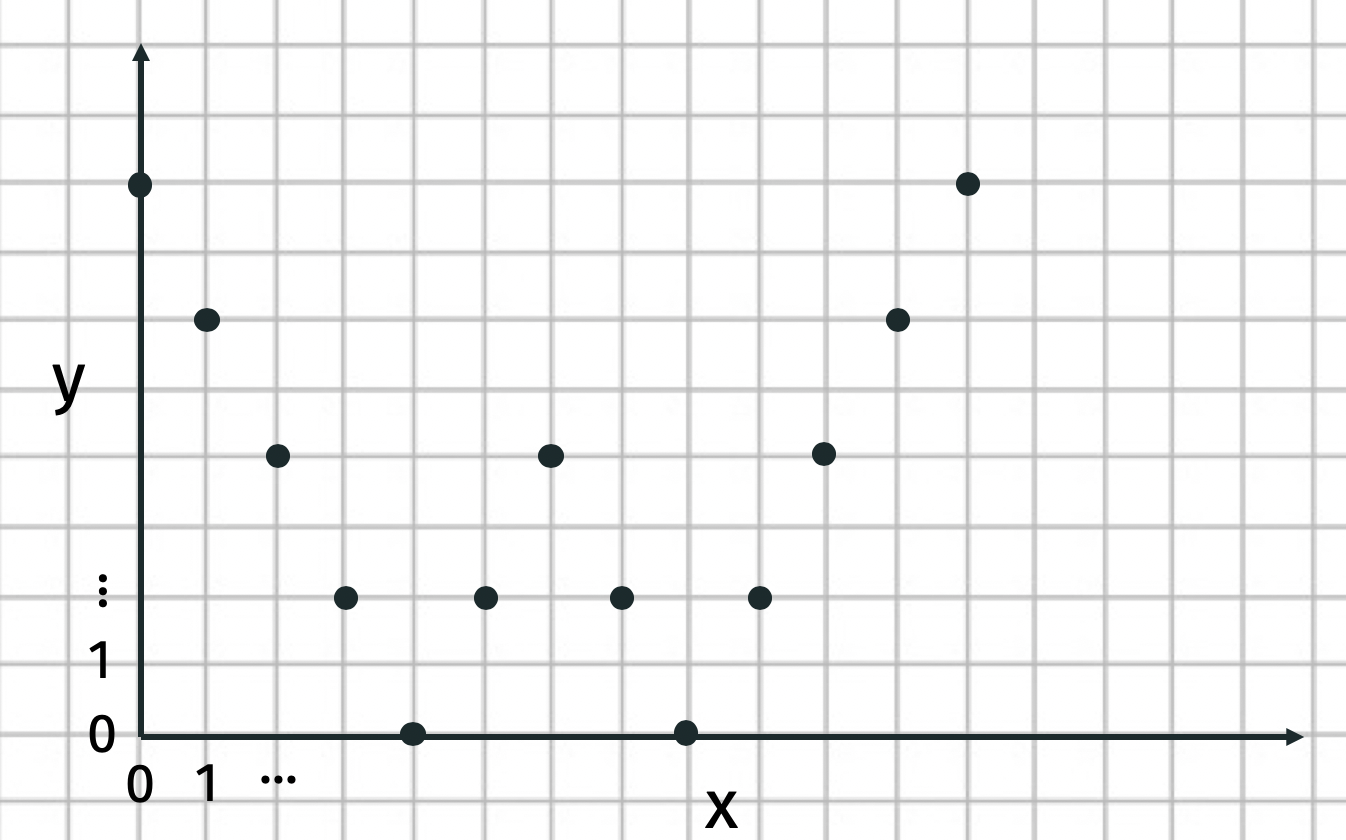
\includegraphics[width=\textwidth]{data_2.png}
			\caption{Dataset 1}
		\end{subfigure}
	~
		\begin{subfigure}{0.45\textwidth}
			\centering
			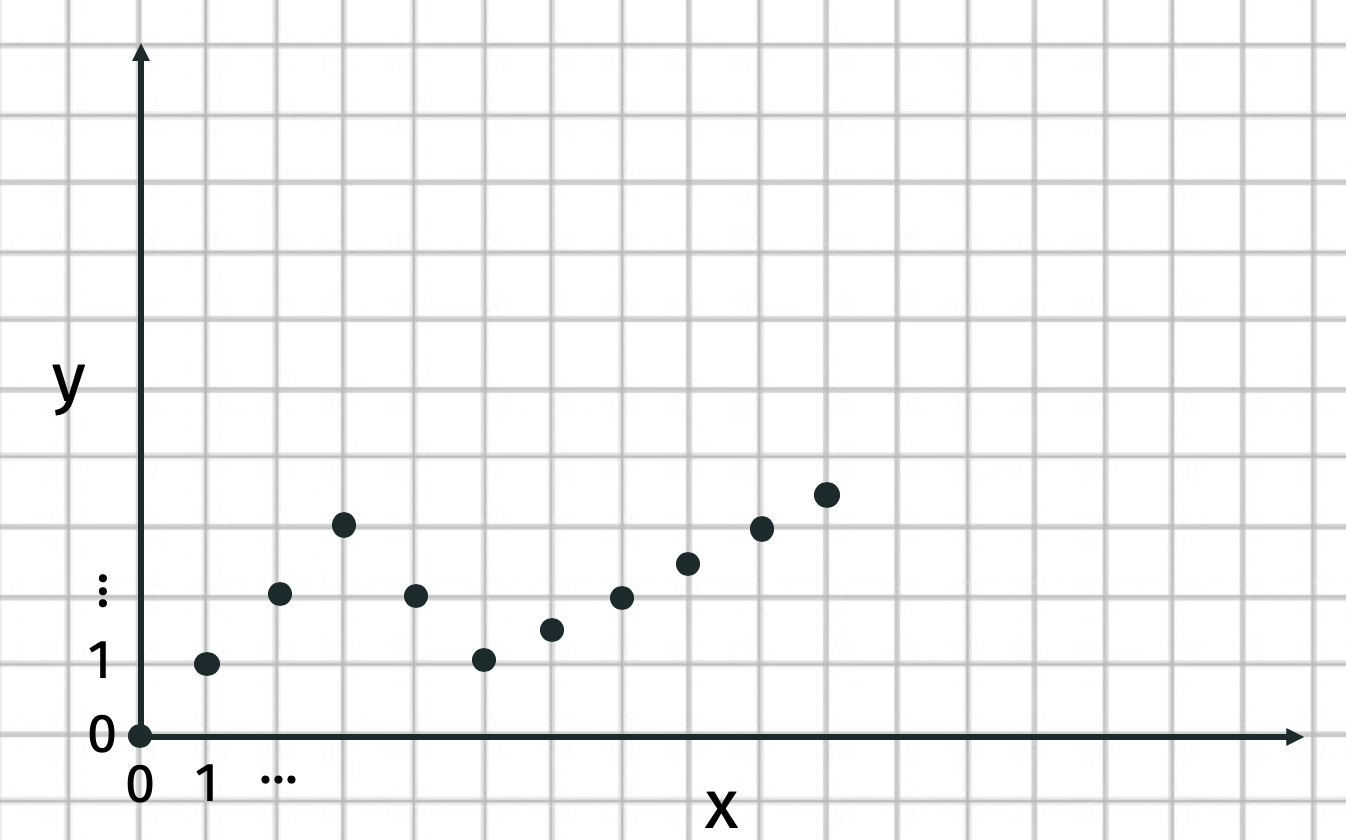
\includegraphics[width=\textwidth]{data_1.png}
						\caption{Dataset 2}
		\end{subfigure}
	\end{figure}
	
	\item For input parameters $\vec{\theta}$ let $f(x,\vec{\theta})$ denote the output of the neural network for a given input $x$. We want to train the network under the squared loss. Specifically, given a training dataset $(x_1,y_1),\ldots, (x_n,y_n)$, we want to choose $\vec{\theta}$ to minimize the loss:
	\begin{align*}
	\mathcal{L}(\vec{\theta}) = \sum_{i=1}^n (y_i - f(x_i,\vec{\theta}))^2.
	\end{align*}
	Write down an expression for the gradient $\nabla \mathcal{L}(\vec{\theta})$ in terms of $\nabla f(x_1,\vec{\theta}), \ldots, \nabla f(x,\vec{\theta})$. \textbf{Hint:} Use chain rule.

	\item Suppose we randomly initialize the network with $\pm 1$ random numbers:
	\begin{align*}
	W_{H,1} = -1, W_{H,2} = 1 , W_{H,3} = 1, W_{H,4} = -1\\
	b_{H,1} = 1, b_{H,2} = 1,b_{H,3} = -1,b_{H,4} = 1 \\
	W_{O,1} = -1, W_{O,2} = -1 , W_{O,3} = -1, W_{O,4} = 1\\
	b_O = 1
	\end{align*}
	Call this initial set of parameter $\vec{\theta}_0$. Use forward-propagation to compute $ f(x,\vec{\theta}_0)$ for $x = 2$. 
	
	\item Use back-propagation to compute $\nabla f(x,\vec{\theta}_0)$ for $x = 2$. To do the computation you will need to use the derivative of the ReLU function, $\max(0,z)$. You can simply use:
	\begin{align*}
	\frac{\partial}{\partial z} \max(0,z) = \begin{cases}
	0 &\text{if } z \leq 0\\
	1 &\text{if } z > 0
	\end{cases}
	\end{align*}
	This derivative is discontinuous, but it turns out that is fine for use in gradient descent.
\end{enumerate}

\end{document}